
\begin{landscape}

\begin{figure}[hp]
\centering
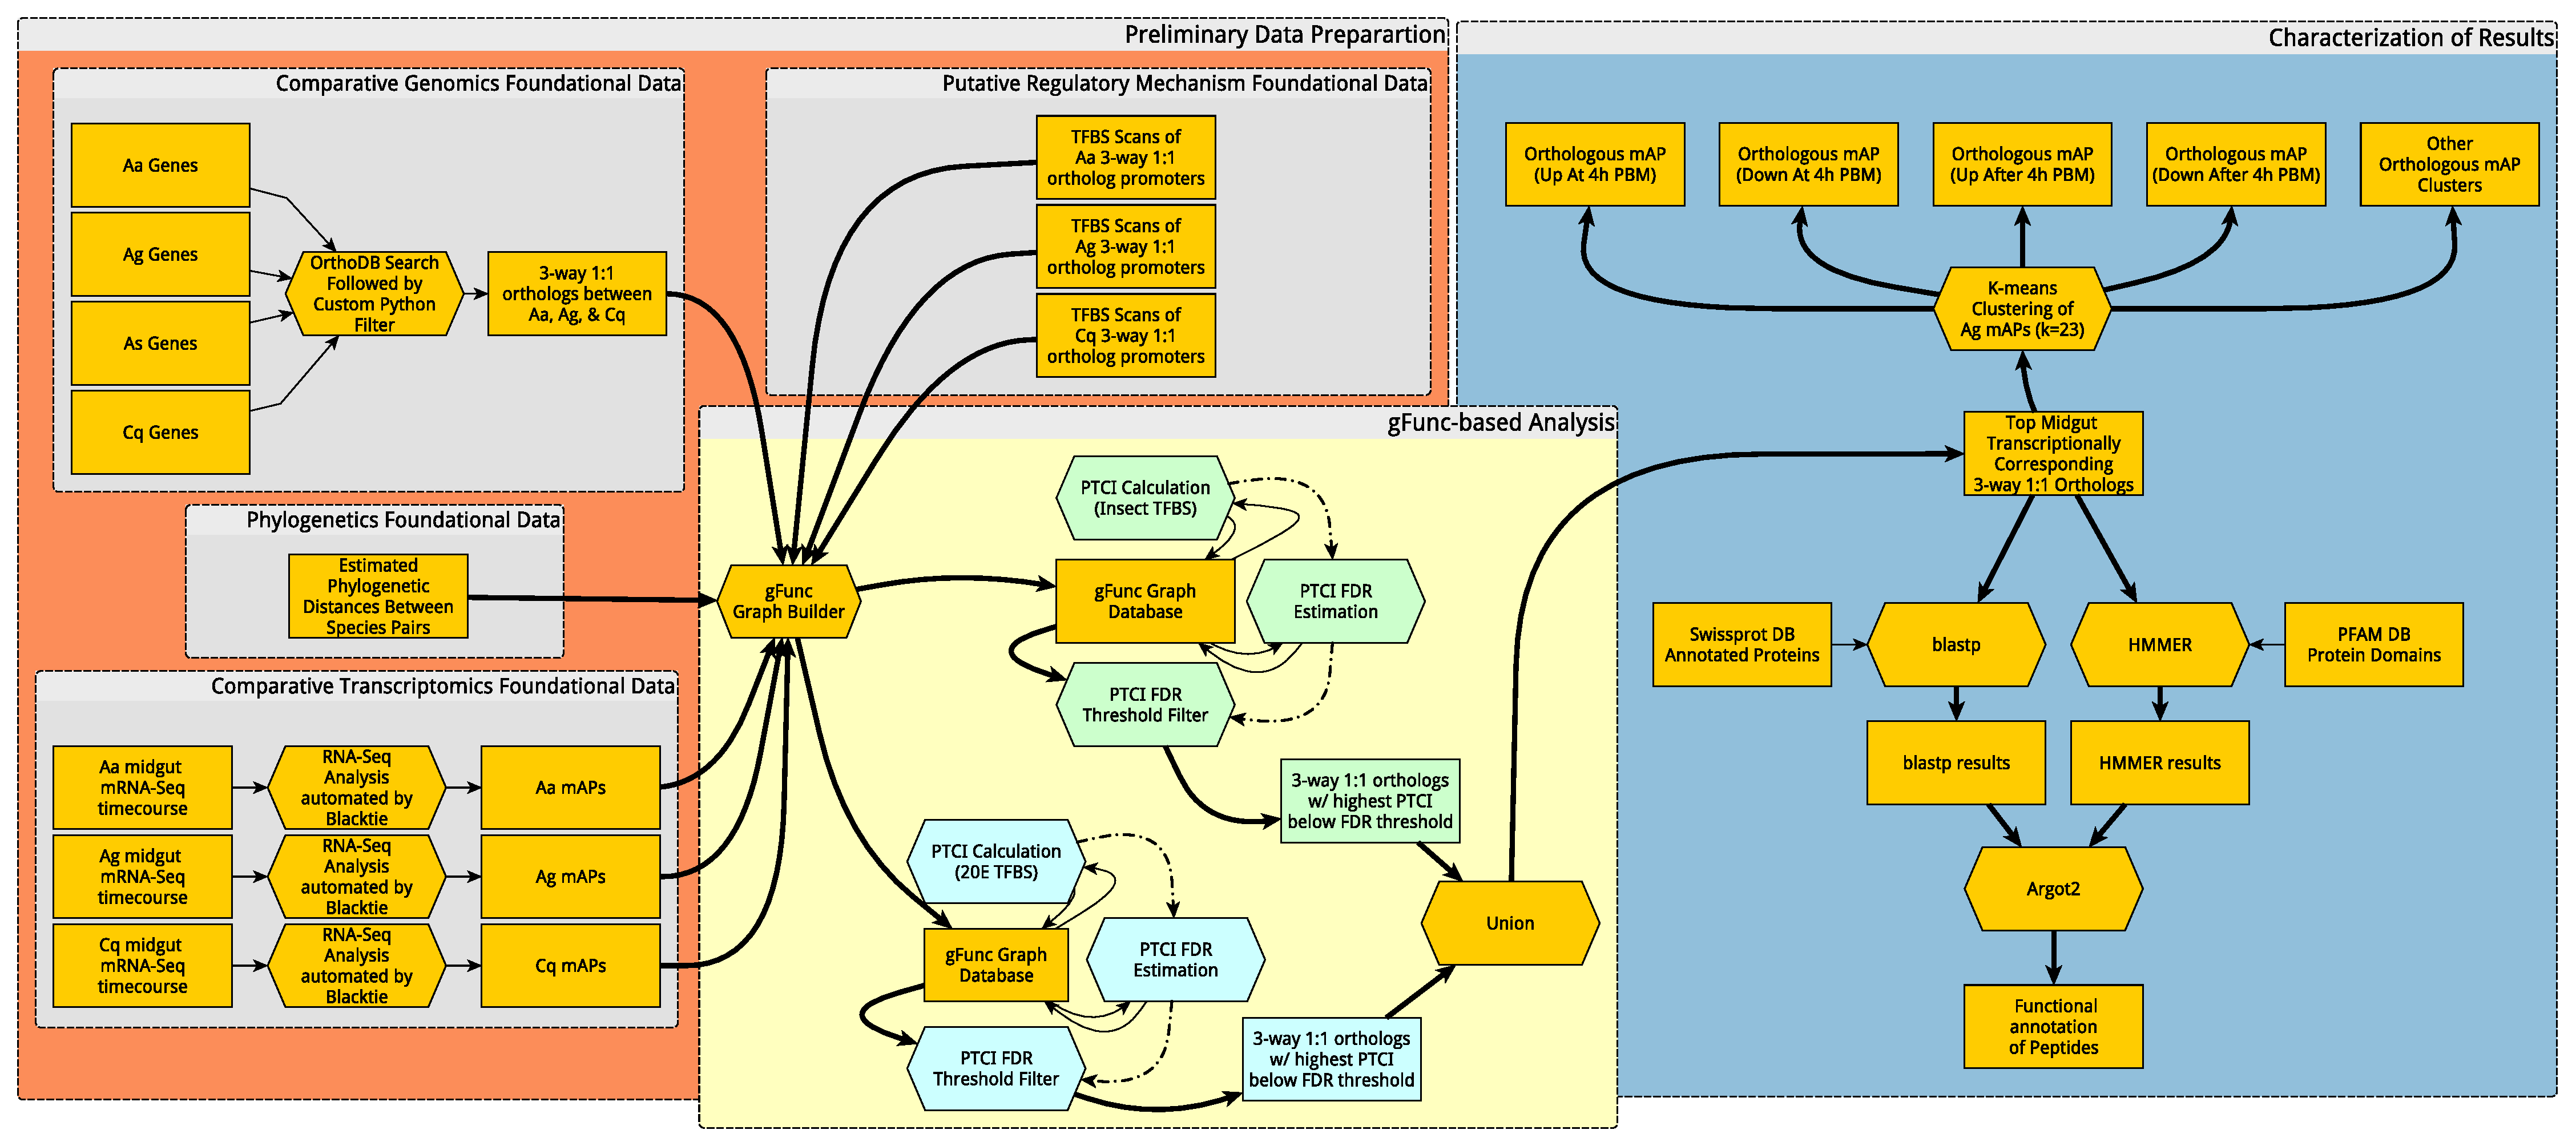
\includegraphics[width=\linewidth]{figures/figs/approach_chart/approach_overview.pdf}

\caption[Input-output diagram of approach overview]{
\sf \textbf{Input-output diagram of approach overview:}
%
The approach employed can be divided into three stages.
\textsc{Preliminary Data Preparation }consists of accumulating and preparing the foundational data representing the four data-types to be integrated into the \gls{gFunc} graph.
\textsc{gFunc-based Analysis} involves mapping the foundational data onto the gFunc graph structure and submitting the graph to custom Python functions that read, analyze, and write results back to the graph to calculate the \glspl{PTCI} and corresponding \glspl{FDR}.
This is done using two \gls{TFBS} profile data-sets with results being merged by a union-type set-operation to obtain the overall set orthologs representing putatively conserved midgut \glspl{mAP}.
\textsc{Characterization of Results} then uses \gls{Argot2} \cite{Falda2012} to obtain functional annotations of the ortholog-sets, and the \glspl{mAP} of \Ag\ members are clustered using k-means clustering to group the ortholog-sets by expression similarity.


\textsc{Heavy Arrows:} main flow of data \\
\textsc{Light Arrows:} preliminary or minor data flow \\
\textsc{Dashed Arrows:} disambiguation of execution order \\
\textsc{Square Node:} data set \\
\textsc{Hexagon Node:} analysis operation

}
\label{fig:approach-chart}
\end{figure}

\end{landscape}